%%%%%%%%%%%%%%%%%%%%%%%%%%%%%%%%%%%%%%%%%%%%%%%%%%%%%%%%%%%%%%%
%
% Welcome to Overleaf --- just edit your LaTeX on the left,
% and we'll compile it for you on the right. If you open the
% 'Share' menu, you can invite other users to edit at the same
% time. See www.overleaf.com/learn for more info. Enjoy!
%
%%%%%%%%%%%%%%%%%%%%%%%%%%%%%%%%%%%%%%%%%%%%%%%%%%%%%%%%%%%%%%%
\documentclass{beamer}
\usepackage{tikz}
\usepackage{amsmath, bm, amssymb}
\usepackage{graphicx}
\usepackage{xcolor}
\usepackage{hyperref}
\usepackage{algorithm}
\usepackage[noend]{algpseudocode}
\hypersetup{
    colorlinks=true,
    linkcolor=blue,
    filecolor=magenta,
    urlcolor=cyan,
    }
\usepackage[backend=biber, citestyle=authoryear, bibstyle=alphabetic]{biblatex}
\addbibresource{bibliography.bib}



\usepackage{tikzsymbols}
\usetheme{Frankfurt}
\usecolortheme{seahorse}
\newcommand{\thetab}{\boldsymbol{\theta}}
\newcommand{\xb}{\boldsymbol{x}}
\DeclareMathOperator*{\argmin}{arg\,min}
\DeclareMathOperator*{\argmax}{arg\,max}

\title[FUB-Presentation]{Bayesian Inference and Explainable AI}
\subtitle{Quantifying the uncertainty of the explanations}
\author[Gkolemis, Vasilis] % (optional)
{Vasilis Gkolemis\inst{1}}

\institute[VFU] % (optional)
{
  \inst{1}%
  ATHENA Research and Innovation Center
}

\date{November 2021}


% Use a simple TikZ graphic to show where the logo is positioned
% \logo{\begin{tikzpicture}
% \filldraw[color=red!50, fill=red!25, very thick](0,0) circle (0.5);
% \node[draw,color=white] at (0,0) {LOGO HERE};
% \end{tikzpicture}}

%End of title page configuration block
%------------------------------------------------------------
%The next block of commands puts the table of contents at the
%beginning of each section and highlights the current section:

\AtBeginSection[]
{
  \begin{frame}
    \frametitle{Program}
    \tableofcontents[currentsection]
  \end{frame}
}

% ------------------------------------------------------------
\begin{document}
\frame{\titlepage}
%---------------------------------------------------------



% chapter 1
\section{Bayesian Formulation}
\subsection{Differences with traditional ML}
\begin{frame}
  \frametitle{Traditional Machine Learning}
  \begin{itemize}
    \item Parametric model \( f_{\thetab}: \xb \rightarrow y \)
    \item Define a distance function \( d(\cdot, \cdot) \) and measure the
          distance (loss) from observed data
      \begin{equation}
        L(\thetab) = \sum_i^N d(f_{\thetab}(\xb^i), y^i)
      \end{equation}
    \item Search for the parameter set $\hat{\thetab}$ that reproduces the observed data best
      \begin{equation}
         \hat{\thetab} = \argmin_{\thetab} L(\thetab)
      \end{equation}
    \end{itemize}
    \noindent\makebox[\linewidth]{\rule{\paperwidth}{0.4pt}}
    We search for a \alert{single configuration (point-estimate) \( \hat{\thetab}\) }

\end{frame}

\begin{frame}
  \frametitle{Bayesian Formulation}
  \begin{itemize}
    \item On the modelling part:
      \begin{itemize}
        \item we need the \textcolor{blue}{joint distribution \(p(\xb,y,\thetab)\)}
        \item to replace the \textcolor{red}{parametric model \(f_{\thetab}: \xb \rightarrow y\)}
      \end{itemize}

    \item Training part:
      \begin{itemize}
        \item infer the \textcolor{blue}{posterior distribution \(p(\thetab|D)\)}
        \item to replace the optimal \textcolor{red}{point estimate \(\hat{\thetab} = \argmin_{\thetab} L(\thetab)\)}
      \end{itemize}

    \item Prediction part:
      \begin{itemize}
        \item infer the \textcolor{blue}{predictive distribution \(p(y|\xb,D)\)}
        \item to replace the \textcolor{red}{point-estimate prediction \(y=f_{\hat{\thetab}}(\xb)\)}
      \end{itemize}
    \end{itemize}
    \noindent\makebox[\linewidth]{\rule{\paperwidth}{0.4pt}}
    We replace point estimates \alert{with distributions (uncertainty quantification)}

\end{frame}

\begin{frame}
  \frametitle{Modelling part}
  \begin{itemize}
    \item joint distribution \( p(\xb, y, \thetab) = p(y|\xb,\thetab) p(\xb) p(\thetab) \)
    \item \( p(\thetab) \), our prior belief about the parameters of the model
    \item \( p(y|\xb, \thetab)\), the likelihood of the model
    \item joint distribution can be defined as a \alert{DAG}
  \end{itemize}

  \begin{figure}[!h]
  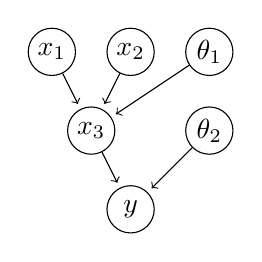
\begin{tikzpicture}[scale=.3]
  \node (x1) [draw, circle, xshift=0cm, minimum size=.6cm, inner sep=0pt]{$x_1$};
  \node (x2) [draw, circle, xshift=0cm, right of=x1, minimum size=.6cm, inner sep=0pt] {$x_2$};
  \node (th1) [draw, circle, xshift=0cm, right of=x2, minimum size=.6cm, inner sep=0pt] {$\theta_1$};
  \node (x3) [draw, circle, xshift=-.5cm, below of=x2, minimum size=.6cm, inner sep=0pt] {$x_3$};
  \node (th2) [draw, circle, xshift=1cm, below of=x2, minimum size=.6cm, inner sep=0pt] {$\theta_2$};
  \node (y) [draw, circle, xshift=.5cm, below of=x3, minimum size=.6cm, inner sep=0pt] {$y$};

  \draw [->, shorten >=2pt] (x1) -- (x3);
  \draw [->, shorten >=2pt] (x2) -- (x3);
  \draw [->, shorten >=2pt] (th1) -- (x3);
  \draw [->, shorten >=2pt] (x3) -- (y);
  \draw [->, shorten >=2pt] (th2) -- (y);
  \end{tikzpicture}
\end{figure}

\noindent\makebox[\linewidth]{\rule{\paperwidth}{0.4pt}}
\begin{itemize}
\item We need to model \alert{ \(p(\thetab) \text{ and } p(y|\xb, \thetab) \)}
\end{itemize}

\end{frame}


\begin{frame}
  \frametitle{Training part}
  \begin{itemize}
  \item We use Bayes law to infer the posterior distribution
    \begin{equation}
      p(\thetab|D) = \frac{p(D|\thetab)p(\thetab)}{p(D)} \propto \prod_i^N p(y^i|\xb^i, \thetab)p(\thetab)
    \end{equation}
    where $D = \{\xb^i, y^i\}_{i=\{1, ..., N\}}$, the observed data (training-set)
    \item In the extreme case where $p(\thetab|D) = \delta(\thetab - \hat{\thetab})$, we get a point-estimate is in traditional ML
    \end{itemize}

    \noindent\makebox[\linewidth]{\rule{\paperwidth}{0.4pt}}
    The `training process` leads to many possible models, each one with different probability (\alert{uncertainty about the model})

\end{frame}

\begin{frame}
  \frametitle{Inference part}
  \begin{itemize}
  \item We need to solve/approximate the predictive distribution $p(y|\xb, D) = \int_{\thetab} p(y|\xb,\thetab)p(\thetab|D) \partial \thetab$
  \item We consider the posterior $p(\thetab|D)$ as known (computed exactly or approximated)
  \item In the extreme case where
    $p(\thetab|D) = \delta(\thetab - \hat{\thetab})$, we get all the mass of the
    prediction $p(y|\xb, D) = p(y|\xb,\hat{\thetab})$ from a single model
  \end{itemize}

    \noindent\makebox[\linewidth]{\rule{\paperwidth}{0.4pt}}
  The `prediction process` gets one prediction per each
    plausible model (\alert{uncertainty about the model leads to uncertainty about the
    prediction})


\end{frame}

\subsection{Pros and Cons}
\begin{frame}
  \frametitle{Bayesian Formulation - Disadvantages}
  What we lose
  \begin{itemize}
  \item On the modelling part
    \begin{itemize}
    \item Time to think how the input features $x_i$ relate to each
      other i.e. building the DAG
    \end{itemize}
    \item On the training-prediction (inference) part
      \begin{itemize}
        \item Expressions difficult to approximate
        \item $p(\thetab|D)$ - how to compute the posterior distribution?
        \item $p(y|\xb,D) = \int_{\thetab} p(y|\xb, \thetab) p(\thetab|D)\partial \thetab$ - how to compute the predictive distribution?
      \end{itemize}
    \end{itemize}
\noindent\makebox[\linewidth]{\rule{\paperwidth}{0.4pt}}
Bayesian Formulation is \alert{difficult from both the mathematical and the computational point-of-view}
\end{frame}

\begin{frame}
  \frametitle{Bayesian Formulation - Advantages}
  What we get:
  \begin{itemize}
  \item On the modelling part
    \begin{itemize}
    \item Specify who the features relate to each other
    \item check \href{https://www.mbmlbook.com/}{Model-based Machine Learning} - a new approach for ML model building
    \end{itemize}
  \item On the inference part
    \begin{itemize}
    \item Uncertainty estimation! Why we need it?
    \item Most times the available data is not enough to reveal a single instance $\hat{\thetab}$
    \item Sometimes we want to predict on a new $\xb$ that is very
      different from the training set
    \end{itemize}
  \end{itemize}
\noindent\makebox[\linewidth]{\rule{\paperwidth}{0.4pt}}
\alert{Let's be wise enough and be uncertain about our predictions.}
\end{frame}


\begin{frame}

  \frametitle{Bayesian Formulation - Example}  \begin{itemize}
    \item In areas without training points our uncertainty is bigger
  \end{itemize}


  \begin{figure}[ht]
    \centering
    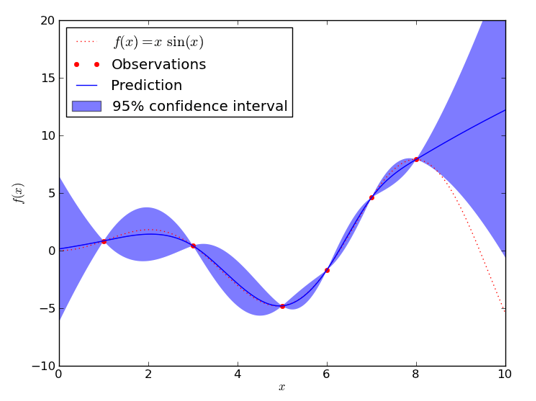
\includegraphics[scale=0.5]{./images/gp.png}
    \label{fig:bayesian_predictive}
  \end{figure}
\end{frame}


% chapter 2
\section{MSc Dissertation - UoE 2020}
\begin{frame}
  \frametitle{Overview of my MSc Dissertation}
  \begin{itemize}
  \item In BI, estimating the posterior is the major difficult task
  \item Remember, \( posterior \propto likelihood * prior \)
  \item When the likelihood is intractable \( \rightarrow\) Likelihood-free inference (LFI) methods
  \item That was my MSc about:
    \begin{itemize}
    \item Extending ROMC, a likelihood-free inference method
    \item Initial paper by~\cite{Ikonomov2020RobustOM}
    \item Implementing ROMC ELFI, a python package for LFI
    \item \href{https://elfi.readthedocs.io/en/latest/}{https://elfi.readthedocs.io/en/latest/}    \end{itemize}
  \end{itemize}

  \noindent\makebox[\linewidth]{\rule{\paperwidth}{0.4pt}}
  LFI methods approximate the posterior when the likelihood is intractable - \alert{very difficult problem}
\end{frame}

\subsection{Likelihood-free inference methods}

\begin{frame}
  \frametitle{Cases of intractable likelihood}
  \begin{itemize}
    \item What causes an intractable likelihood?
    \begin{itemize}
    \item Many reasons (e.g. intractable partition functions in unnormalized statistical models)
    \item Most common reason \( \rightarrow \) \alert{unobserved/latent variables}
    \item Latent variables are really important in many modelling cases (example in next slide)
    \end{itemize}
  \item Simulator-based models (those with intractable likelihood) are widely-used in natural sciences i.e. biology, epidemiology, neuroscience
    \item An overview of the field in \cite{Cranmer30055}

    \end{itemize}
\noindent\makebox[\linewidth]{\rule{\paperwidth}{0.4pt}}
Simulator-based models provide valuable \alert{modelling freedom}
\end{frame}

\begin{frame}
  \frametitle{Example of intractable likelihood (1)}
\begin{itemize}
  \item Predict the grade $y$ of a candidate at an important test
  \item Grade is a direct consequence of two things
  \begin{itemize}
    \item $u_1 \in [0,10]$ the mental readiness of the candidate
    \item $u_2 \in [0,10]$ the knowledge of the topic
  \end{itemize}
\item the mental readiness is direct consequence of
  \begin{itemize}
  \item $x_1$ how many hours he has slept the previous night
  \item $x_2$ how many times he has been in stressful exams in the past
  \end{itemize}
\item knowledge of the topic
  \begin{itemize}
  \item $x_3$, years of experience in software engineering
  \item $x_4$, number of application he has developed
  \end{itemize}
\end{itemize}
  \noindent\makebox[\linewidth]{\rule{\paperwidth}{0.4pt}}
  Think more about it; \alert{it is sensible to model the latent variables!}
\end{frame}


\begin{frame}
  \frametitle{Example of intractable likelihood (2)}
  \begin{itemize}
    \item \( L(\thetab) = p(D|\thetab) \propto \prod_i^N p(y^i|x^i, \thetab) = \int_{u_1,u_2}p(y^i, u^i|x^i, \thetab) \)
    \item The likelihood is defined over an integral - intractable in the general case
    \item But sampling is feasible i.e. draw \( y \sim p(y|x, \thetab) \)
  \end{itemize}

  \begin{figure}[!h]
  \tikzstyle{observable} = [draw, circle, minimum size=.6cm, inner sep=0pt,
    fill=black!30!green]
  \tikzstyle{latent} = [draw, circle, minimum size=.6cm, inner sep=0pt]
  \begin{tikzpicture}[scale=.3]
  \node (x1) [observable, xshift=0cm]{$x_1$};
  \node (x2) [observable, xshift=0cm, right of=x1] {$x_2$};
  \node (x3) [observable, xshift=0cm, right of=x2] {$x_3$};
  \node (x4) [observable, xshift=0cm, right of=x3] {$x_4$};
  \node (u1) [latent, xshift=-.5cm, below of=x2] {$u_1$};
  \node (u2) [latent, xshift=.5cm, below of=x3] {$u_2$};
  \node (y) [observable, xshift=1cm, below of=u1] {$y$};

  \draw [->, shorten >=2pt] (x1) -- (u1);
  \draw [->, shorten >=2pt] (x2) -- (u1);
  \draw [->, shorten >=2pt] (x3) -- (u2);
  \draw [->, shorten >=2pt] (x4) -- (u2);
  \draw [->, shorten >=2pt] (u1) -- (y);
  \draw [->, shorten >=2pt] (u2) -- (y);
  \end{tikzpicture}
\end{figure}

\noindent\makebox[\linewidth]{\rule{\paperwidth}{0.4pt}}
If we want latent variables, we \alert{have to use likelihood-free methods.}

\end{frame}

\subsection{Robust Optimization Monte Carlo (ROMC)}

\begin{frame}
  \frametitle{Optimization Monte Carlo (OMC)}
  \begin{itemize}
    \item Core idea: \alert{Convert random sampling to a deterministic process} \cite{NIPS2015_a284df11}
      \begin{equation}
        x \sim p(x|\thetab) \Rightarrow f(\thetab, v) \rightarrow x
      \end{equation}

      \item $v$ is the nuisance variable that absorbs all the randomness
      \item $\argmax_{\thetab} p(x=x_0|\thetab) \rightarrow \argmin_{\thetab}|f(\thetab, v=v_0) - x_0| $
      \item In a computer program, the value that governs all randomness is the random seed
  \end{itemize}

  \noindent\makebox[\linewidth]{\rule{\paperwidth}{0.4pt}}
  Maximizing the probability of generating some data can be converted to a \alert{deterministic optimization process}
\end{frame}

\begin{frame}
  \frametitle{Robust Optimization Monte Carlo (ROMC), step (1)}
  \begin{itemize}
  \item What is the objective? A way to approximate the intractable $L(\thetab)=p(D|\thetab)$
  \item What I have? Only a way to simulate points from
    $p(y|\xb, \thetab)$ (random simulator)
  \item Draw random seeds $s$ and generate deterministic simulators $f_i(\thetab)$
  \item For every $f_i$, search for the
    $\thetab_i^* = argmin_{\thetab} |f_i(\thetab) - D|$
  \item For every $f_i$, define an area $\mathcal{S}_i$ around
    $\thetab_i^*$ such that $|f_i(\thetab) - D| < \epsilon$
  \item $\mathcal{S}_i$ is the acceptance region of the $i-th$ simulator
  \end{itemize}

  \noindent\makebox[\linewidth]{\rule{\paperwidth}{0.4pt}}
  Convert random sampling to an optimization process and find the parameters $\thetab_i$ that generate data close to the observations.

\end{frame}

\begin{frame}
  \frametitle{Robust Optimization Monte Carlo (ROMC), step (2)}
  \begin{itemize}
  \item The approximate posterior is the sum of all such regions $S_i$, scaled by the prior
    \begin{equation}
      p(\thetab|D) \approx p(\thetab) \frac{1}{N} \sum_i \mathcal{S}_i(\thetab)
    \end{equation}
    where $\mathcal{S}_i(\thetab) = \frac{1}{V}$ if $|f_i(\thetab) - D| < \epsilon$, otherwise $0$
  \item Each point inside the area is equally probable to have generated the data
  \end{itemize}

  \noindent\makebox[\linewidth]{\rule{\paperwidth}{0.4pt}}
  The posterior approximation is the sum of all the regions $\mathcal{S}_i(\thetab)$ that generate data close to the observations. (as in typical loss minimization)
\end{frame}


\begin{frame}
  \frametitle{An example of an acceptance region}
  \begin{figure}[ht]
    \begin{center}
        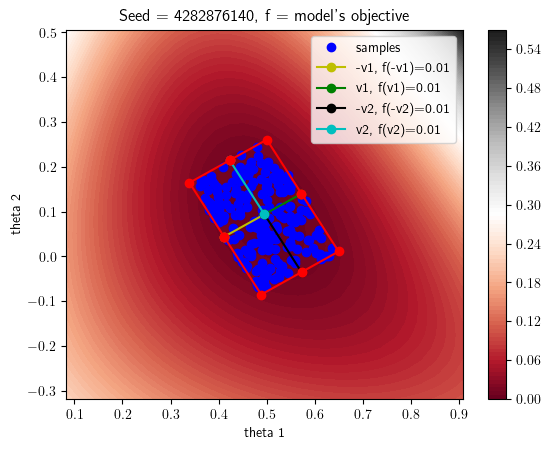
\includegraphics[width=0.55\textwidth]{./images/chapter4/ma2_region_1.png}
    \end{center}
  \caption[The acceptance region of a specific deterministic simulator.]{The acceptance region $S_i$ of a specific optimisation problem, that will contribute to the posterior.}
  \label{fig:ma2_5}
\end{figure}
\end{frame}

\begin{frame}
  \frametitle{ROMC - Training/Fitting part}
  \begin{algorithmic}[1]
    \Procedure{ROMC}{}
    \For{$i \gets 1 \textrm{ to } n_1$}
      \State $\mathbf{v}_i \sim p(\mathbf{v})$ \Comment{Draw nuisance variables}
      \State $f_i(\thetab)$ \Comment{Define deterministic simulator}
      \State $\thetab_i^* = \text{argmin}_{\thetab} |f_i(\thetab) - D|$ \Comment{Solve optimization problem}
      \If{$|f_i(\thetab) - D| > \epsilon$}
        \State Go to 2 \Comment{Filter solution}
      \EndIf
      \State Define the proposal area $\mathcal{\hat{S}}_i$ \Comment{Estimate proposal area}
    \EndFor
    \EndProcedure
  \end{algorithmic}

  \noindent\makebox[\linewidth]{\rule{\paperwidth}{0.4pt}}
  Algorithmic view of the training part of ROMC
\end{frame}

\begin{frame}
  \frametitle{ROMC - Training part (Recap)}

  \begin{itemize}
  \item Target of Bayesian Inference
    \begin{itemize}
    \item infer the \textcolor{blue}{posterior distribution $p(\thetab|D)$}
    \end{itemize}
  \item ROMC proposal
    \end{itemize}
    \begin{equation}
      p(\thetab|D) \approx p(\thetab) \frac{1}{N} \sum_i \mathcal{S}_i(\thetab)
    \end{equation}

    \begin{itemize}
    \item where
      \begin{itemize}
      \item $\mathcal{S}_i(\thetab) = \frac{1}{V}$ if $|f_i(\thetab) - D| < \epsilon$, otherwise $0$
      \item $V$ is the volume of $\mathcal{S}_i(\thetab)$
      \end{itemize}
    \end{itemize}
  \noindent\makebox[\linewidth]{\rule{\paperwidth}{0.4pt}}
  ROMC approximation of the posterior distribution using only the simulator
\end{frame}

\begin{frame}
  \frametitle{ROMC - Prediction part}
  \begin{algorithmic}[1]
    \\\hrulefill
    \Procedure{ROMC}{}
    \For{$i \gets 1 \textrm{ to } n_1$}
        \For{$j \gets 1 \textrm{ to } n_2$}
        \State $\thetab_{ij} \sim q_i$, compute $w_{ij}$ \Comment{Sample}
      \EndFor
    \EndFor
    \State $E_{p(\thetab|D)}[h(\thetab)]$ \Comment{Estimate an expectation}
    \State $p_{d,\epsilon}(\thetab)$ \Comment{Evaluate the unnormalized posterior}
    \\\hrulefill
    \EndProcedure
  \end{algorithmic}
  \noindent\makebox[\linewidth]{\rule{\paperwidth}{0.4pt}}
  Algorithmic view of the prediction part of ROMC; how to sample from the posterior and
  estimate an expectation.

\end{frame}

\begin{frame}
  \frametitle{ROMC - Prediction part}
  \begin{itemize}
  \item Target of Bayesian Inference
    \begin{itemize}
    \item infer the \textcolor{blue}{predictive distribution $p(y|x,D)$}
    \end{itemize}
  \item ROMC proposal
    \begin{itemize}
    \item Sample from each samples from each acceptance region $(w_{ij}, \thetab_{ij})$
      \item Normalize them to sum to one $w_{ij} = \frac{1}{\sum_j w_{ij}}$
      \item $p(y|x, D) \approx \sum_i \sum_j w_{ij}f_i(\thetab, x)$
      \end{itemize}
    \end{itemize}
  \noindent\makebox[\linewidth]{\rule{\paperwidth}{0.4pt}}
  ROMC approximation of the predictive distribution using only the simulator

\end{frame}

\begin{frame}
  \frametitle{ROMC - Advantages}
  \begin{itemize}
  \item Efficient and Embarrassingly Parallel Framework for likelihood-free inference
  \item \alert{Efficient}, because it turns every random-generating
    process to a deterministic optimization problem \( \Rightarrow \)
    does not spend samples unreasonably
  \item \alert{Embarrassingly Parallel}, all optimisation processes
    can run in parallel \( \Rightarrow \) super-fast if many cores are accesible
  \item \alert{Framework}, because is a general recipe. The components
    that will be used depend on the user e.g. gradient-based optimizer
    or bayesian optimization
  \end{itemize}
  \noindent\makebox[\linewidth]{\rule{\paperwidth}{0.4pt}}
  ROMC is efficient and parallelizable.
\end{frame}

\subsection{Implementation at ELFI}
\begin{frame}
  \frametitle{Implementation at ELFI}
  \begin{itemize}
  \item Fully parallelizable and extendable implementation at ELFI
  \item \href{https://elfi.readthedocs.io/en/latest/}{https://elfi.readthedocs.io/en/latest/}
  \item Interactive jupyter notebooks with examples (google colab - no need for installing anything)
  \begin{itemize}
  \item \href{https://colab.research.google.com/drive/1lGRp0XrNfZ64NN0ASB_tYEKowXwlveDC}{Simple 1D example}
  \item \href{https://colab.research.google.com/drive/1Fof_WmCi1YizzSI_63aEsbLXsno5gSZ3}{Simple 2D example}
  \item \href{https://colab.research.google.com/drive/1nkdACQ370SSc0KB1bHv4sBRaxMlMqoNH}{Moving Average example}
  \item \href{https://colab.research.google.com/drive/1RzB-V1QueP1y1nyzv_VOqR1nVz3DUH3v}{Tutorial for extending the ROMC method with a Neural Network}
  \end{itemize}
  \item Paper about to be submited at JSS
  \end{itemize}
  \noindent\makebox[\linewidth]{\rule{\paperwidth}{0.4pt}}
  Feel-free to experiment with ROMC
\end{frame}


\subsection{Future Ideas}

\begin{frame}
  \begin{itemize}
  \item Find ways to make it efficient in high dimensional parametric
    space ( \(\approx 20 \) is high for LFI methods)
  \item Implement ROMC in a package with automatic differentiation, to
    see how it scales in higer-dimensions
  \item JAX a good candidate, provides novel way to freeze the seed
    without global side-effects
  \item Research for better (accurate and efficient) ways to estimate
    the regions \( \mathcal{S}_i \) in high-dimensions
  \end{itemize}
  \noindent\makebox[\linewidth]{\rule{\paperwidth}{0.4pt}}
  Stay alert, there will be updates!
\end{frame}

% chapter 3
% \section{Quantify the uncertainty of the Explanations}
% \begin{frame}
  \frametitle{Quantifying the uncertainty of the explanations}
  \begin{itemize}
    \item Many iml methods such as permutation feature importance or
    shaple values provide explanations without quantifying the
    uncertainty of the explanation
    \item The model itself, but also its
    explanations, are computed from data and hence are subject to
    uncertainty
  \item Interpretable Machine Learning – A Brief History,
    State-of-the-Art and Challenges by~\cite{molnar2020interpretable}
  spots it as a major open challenge in XAI domain
\end{itemize}
  \noindent\makebox[\linewidth]{\rule{\paperwidth}{0.4pt}}
  Uncertainty quantification is a major challenge in IML.
\end{frame}

\begin{frame}
  \frametitle{Could Bayesian Reasoning help?}
  \begin{itemize}
  \item We have to (re)define more rigorously the explainablity
    techniques
  \item Remember the two ingredients of Bayesian Reasoning; (a) Modeling
    and (b) Inference
  \item For (a), can we model explainability techniques as
    Probabilistic Graphical Models? (especially local surrogate models)
  \item If achieve (a), we can (re)search for (b) inference techniques
    that will provide explanations with uncertainty estimation
  \end{itemize}
  \noindent\makebox[\linewidth]{\rule{\paperwidth}{0.4pt}}
  Statement we can discuss: Bayesian Reasoning can be a recipe for
  uncertainty estimation in XAI

\end{frame}


\begin{frame}
  \frametitle{Feature effect}
  \begin{itemize}
  \item Some notation
    \begin{itemize}
    \item $x_s$ feature of interest
    \item $\mathbf{x_c}$ the rest of the features
    \item $i$, index pointing to the $i-th$ training example
    \end{itemize}

  \item ALE plots formula:
    \begin{gather}
      y = f_{ALE}(x) = \int_{x_0}^{x} \mathbf{E_{x_c|x_s}[f^{(1)}(x_s=z,x_c)]} \partial z\\
      f^{(1)}(x_s,x_c) =  \frac{\partial f}{\partial x_s}
    \end{gather}
    \item Intuition: \( y = f_{ALE}(x) = \int_{x_0}^{x} (\text{local effect at } z) \partial z \)
    \end{itemize}
  \noindent\makebox[\linewidth]{\rule{\paperwidth}{0.4pt}}
  ALE plots model the feature effect as the \alert{integration of the local feature effects}.

\end{frame}

\begin{frame}
  \frametitle{ALE approximation}
  \begin{itemize}
  \item ALE approximation:
    \begin{gather} \label{eq:ALE_appr}
      \hat{f}_{ALE}(x_s) = \sum_{k=1}^{K_{x_s}} \frac{1}{|N(k)|} \sum_{i:x_s^i \in N(k)} [f(z_k, \mathbf{x_c}^i) - f(z_{k-1}, \mathbf{x_c}^i)]\\
      \text{where} \; N(k) \text{ all the samples that belong to the k-th bin}
    \end{gather}

  \item ALE builds equally-sized bins and approximates the derivative
    by evaluating $f$ at the limits of the bins
  \item Side comment: when bins become large the approximation is bad,
    we work on a better one (stay up to date \dSmiley )
\end{itemize}
  \noindent\makebox[\linewidth]{\rule{\paperwidth}{0.4pt}}
  ALE approximation is weak when bins grow larger.
\end{frame}

\begin{frame}
  \frametitle{Quantify the variance}
  \begin{itemize}
  \item ALE plots formula:
    \begin{gather}
      y = f_{ALE}(x) = \int_{x_0}^{x} \mathbf{E_{x_c|x_s}[f^{(1)}(x_s=z,x_c)]} \partial z\\
      f^{(1)}(x_s,x_c) =  \frac{\partial f}{\partial x_s}
    \end{gather}
  \item ALE plots uses only with the expected local effect $\mathbf{E_{x_c|x_s}[f^{(1)}(x_s=z,x_c)]}$
  \item Intuition: \( y = f_{ALE}(x) = \int_{x_0}^{x} (\text{expected local effect at } z) \partial z \)
  \end{itemize}
  \noindent\makebox[\linewidth]{\rule{\paperwidth}{0.4pt}}
  ALE definition uses only the \alert{expected local effect} at each position
\end{frame}

\begin{frame}
  \frametitle{Quantify the variance}
  \begin{itemize}
  \item In general the local effect is a probability distribution \(p_{eff}(y|x_s)\)
  \item \(p_{eff}(y|x_s) = \int_{x_c} p(y,x_c|x_s) \partial x_c = \int_{x_c} p(y|x_c, x_s) p(x_c|x_s) \partial x_c\)
  \item \( p(y|x_c, x_s) = \delta (y - \frac{\partial f}{\partial x_s}(x_s,x_c)) \)
  \item \( p(x_c|x_s) \) is not known, but there are ways to estimate it?
  \item If estimating the whole distribution \(p_{eff}(y|x_s)\) is difficult, could we at least estimate some critical statistics
    \begin{itemize}
    \item expected value \( \mathbb{E}_{p_{eff}}[y] = \mu \)
    \item Variance \( \mathbb{E}_{p_{eff}}[(y - \mu)^2] \rightarrow \) uncertainty quantification
    \end{itemize}
  \item Details in the paper under construction \dSmiley
  \end{itemize}
  \noindent\makebox[\linewidth]{\rule{\paperwidth}{0.4pt}}
  If model the whole distribution of the local effect, we could estimate the uncertainty of the local effect.
\end{frame}

\begin{frame}
  \frametitle{Some first approaches in the domain}
  \begin{itemize}
  \item Feature importance
    \begin{itemize}
      \item Testing Conditional Independence in Supervised Learning Algorithms\cite{watson2021testing}
      \item All Models are Wrong, but Many are Useful\cite{JMLR:v20:18-760}
      \end{itemize}
    \item Relevance propagation
      \begin{itemize}
      \item On Feature Relevance Uncertainty: A Monte Carlo Dropout Sampling Approach~\cite{fabi2020}
      \end{itemize}
    \item Shapley value
      \begin{itemize}
      \item Efficient nonparametric statistical inference on
        population feature importance using Shapley
        values\cite{williamson2020efficient}
      \end{itemize}
    \end{itemize}
  \noindent\makebox[\linewidth]{\rule{\paperwidth}{0.4pt}}
  The domain of Uncertainty Quantification in XAI is still in its first steps
\end{frame}

\begin{frame}
  Thanks a lot for the attention!

  Let's discuss!
\end{frame}

\begin{frame}[allowframebreaks]
  \frametitle{Bibliography}
  \printbibliography
\end{frame}



\end{document}